\documentclass{beamer}
	\usetheme{Madrid}
	\usecolortheme{beaver}

%%{{{ PACKAGES
\usepackage[utf8]{inputenc}
\usepackage[T1]{fontenc}
\usepackage{lmodern}
\usepackage{couriers}

\usepackage{graphicx}
\usepackage{url}
\usepackage{multicol}
\usepackage{tikz}
	\usetikzlibrary{backgrounds, shapes.geometric, positioning, patterns, external}
	\tikzexternalize

%% Make tikz generate PDF file to .tmp directory
\makeatletter
	\newcommand{\mytikzinput}[1]{%
		\tikzsetnextfilename{tmp/#1}%
	}
\makeatother

\usepackage[
	backend=bibtex
,	style=ieee
]{biblatex}
	\addbibresource{bibliography.bib}

\usepackage{multirow}
\usepackage{datatool}

\usepackage{algorithm}
\usepackage{algpseudocode}

\usepackage{caption}
	\captionsetup{format=hang}
%%}}}

\newcommand{\judul}{%
	Deteksi Vandalisme pada Wikipedia Bahasa Inggris Menggunakan
	Sampel Ulang LNSMOTE
	dan Klasifikasi Cascaded Random Forest
}
\newcommand{\mytitle}{%
	Detecting Vandalism on English Wikipedia using LNSMOTE Resampling and
	Cascaded Random Forest Classifier
}
\newcommand{\myname}{Muhamad Sulhan}
\newcommand{\mysid}{23513014}
\newcommand{\myemail}{ms@students.itb.ac.id}
\newcommand{\myschool}{School of Electrical and Informatics Engineering}
\newcommand{\tfakultas}{Sekolah Teknik Elektro dan Informatika}

\newcommand{\myadvisorname}{Dwi Hendratmo Widyantoro}
\newcommand{\myadvisorshortname}{Dwi H. Widyantoro}
\newcommand{\myadvisorid}{196812071994021001}
\newcommand{\myadvisoremail}{dwi@stei.itb.ac.id}
\newcommand{\mydept}{Program Studi Magister Informatika}

\newcommand{\itb}{Institut Teknologi Bandung}
\newcommand{\itbaddress}{Ganesha 10, Bandung, Indonesia 40132}

\newcommand{\tUpAbstrak}{ABSTRAK}
\newcommand{\tupabstract}{ABSTRACT}
\newcommand{\tuppengesahan}{HALAMAN PENGESAHAN}

\newcommand{\daftarisi}{DAFTAR ISI}
\newcommand{\tupdaftarlampiran}{DAFTAR LAMPIRAN}
\newcommand{\daftargambar}{DAFTAR GAMBAR DAN ILUSTRASI}
\newcommand{\daftartabel}{DAFTAR TABEL}

\newcommand{\tDaftarPustaka}{DAFTAR PUSTAKA}
\newcommand{\tLampiran}{Lampiran}
\newcommand{\tUpLampiran}{\MakeUppercase{\tLampiran}}

%%% My images directory
\graphicspath{{../images/} {images/}}
\newcommand{\myitbcover}{ITB-logo-hitam}
\newcommand{\myitbcoverblue}{ITB-logo-ganesha}


%% remove navigation symbols
\setbeamertemplate{navigation symbols}{}

\title[Detecting Vandalism with CRF]{%
	\mytitle
}
\author{\myname}
\institute[STEI-ITB]{%
	\mydept\\
	\itb
}
\date{2016}
\logo{%
	\includegraphics[width=1cm]{\myitbcoverblue}
}

\begin{document}

\frame{\titlepage}

\section*{Outline}
\begin{frame}
	{Outline}
	\begin{multicols}{2}
		\tableofcontents
	\end{multicols}
\end{frame}

\section{Introduction}

\subsection{What is Vandalism?}
\begin{frame}
	\frametitle{What is vandalism?}
	\begin{definition}
		Willful or malicious destruction or defacement of public or private
		property.
		\footnote{\url{http://www.merriam-webster.com/dictionary/vandalism}}
	\end{definition}
	\pause
	\begin{block}{In the context of Wikipedia}
		Malicious edit which intention is to give wrong information, or hiding
		information by deleting the content, abusive content, ads, and/or
		meaningless text.
	\end{block}
\end{frame}

\subsection{Examples}
\begin{frame}{Example of Vandalism on Wikipedia}{Offensive}
	\begin{figure}
		\centering
		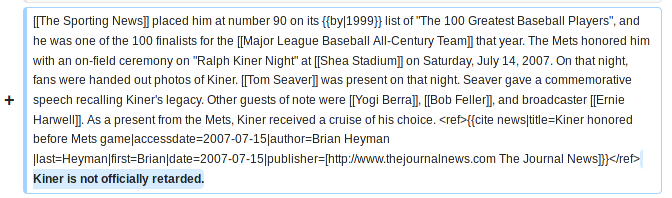
\includegraphics[width=\textwidth]{edit_harassment}
		\caption{
			Harashing public figure.
			(\url{https://en.wikipedia.org/w/index.php?title=Ralph_Kiner&diff=prev&oldid=329569400})
		}
	\end{figure}
\end{frame}

\begin{frame}{Example of Vandalism on Wikipedia}{Meaningless content}
	\begin{figure}
		\centering
		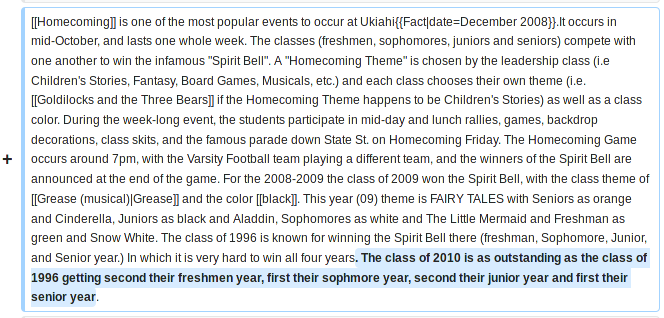
\includegraphics[width=0.7\textwidth]{edit_meaningless}
		\caption{
			The tricky part of detecting vandalism is a well written text but
			having no real importance or value.
			(\url{https://en.wikipedia.org/w/index.php?title=Ukiah_High_School&diff=prev&oldid=329692136})
		}
	\end{figure}
\end{frame}

%%{{{ RELATED WORKS
\subsection{Related Works}

\begin{frame}{Related Works}{What have been done?}
	\begin{block}{Bot}
		A program that check each edit based on,
		\begin{itemize}
		\item blacklist of words
		\item blacklist of IP addresses and users
		\end{itemize}
	\end{block}
	\pause
	\begin{alertblock}{Problems}
		\begin{itemize}
		\item Its not easy to maintain the list
		\item One IP address could be used by many users
		\end{itemize}
	\end{alertblock}
\end{frame}

\begin{frame}{Related Works}{What have been done?}
	\begin{block}{Implementation of machine learning}
		\begin{itemize}
		\item Potthast create and collect the vandalism corpus and the first to
		use machine learning technique to detect vandalism by applying Logistic
		Regression.
		\item Velasco then expand the features by Potthast and use Random
		Forest. Velasco win the 1st International Competition on Wikipedia
		Vandalism Detection. Velasco reach true-positive rate (TPR) value 0.57.
		\item Gotze combines the works of Potthast, Velasco, and others,
		by oversampling the dataset using Synthetic Minority Oversampling
		Technique (SMOTE) and compare several two-class classifiers, including
		Logistic Regression, RealAdaBoost, Random Forest, and Bayesian Network.
		Gotze reach highest TPR value 0.39 with Random Forest.
		\end{itemize}
	\end{block}
\end{frame}
%%}}}

%%{{{ OUR WORKS
\subsection{Our Works}

\begin{frame}{Our Works}
	\begin{itemize}
		\item For resampling, we use an extension of SMOTE proposed by
		Maciejewski and Stefanowski called Local Neighbours SMOTE (LNSMOTE)
		to increase the positive rate.
		\item For classifier, we use Cascaded Random Forest which was
		proposed by Baumann to speeding up the training process and also
		increasing the positive rate.
	\end{itemize}
\end{frame}
%%}}}

\section{Literature Study}

\begin{frame}
	\begin{multicols}{2}
		\tableofcontents[currentsection]
	\end{multicols}
\end{frame}

\subsection{SMOTE}

\begin{frame}{Synthetic Minority Oversampling TEchnique (SMOTE)}
	{Overview}
	\begin{columns}
		\begin{column}{0.5\textwidth}
			\begin{figure}
				\centering
				\mytikzinput{smote_example}
				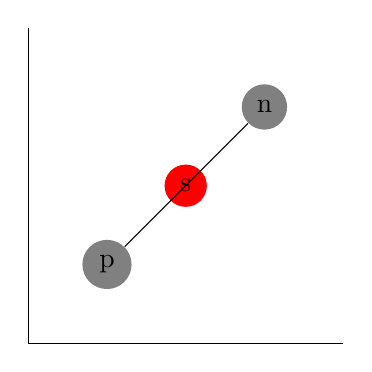
\begin{tikzpicture}
					\draw (0,0) -- (0,4);
					\draw (0,0) -- (4,0);
					\node[circle,fill=gray] (p) at (1,1) {p};
					\node[circle,fill=gray] (n) at (3,3) {n};
					\node[circle,fill=red] (s) at (2,2) {s};
					\draw[-] (p) -- (n);
				\end{tikzpicture}
			\end{figure}
		\end{column}

		\begin{column}{0.5\textwidth}
			Create synthetic sample by substracting feature vector of two
			samples and multiplied it with real random number between 0 and
			1.

			\[
				s = (p - n) * random(0,1)
			\]
		\end{column}
	\end{columns}
\end{frame}

\begin{frame}{Synthetic Minority Oversampling TEchnique (SMOTE)}
	{Problems}
	\begin{columns}
		\begin{column}{0.5\textwidth}
			\begin{figure}
				\mytikzinput{smote_problem_overlapping}
				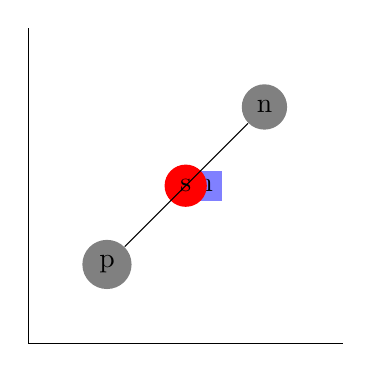
\begin{tikzpicture}
					\draw (0,0) -- (0,4);
					\draw (0,0) -- (4,0);
					\node[circle,fill=gray] (p) at (1,1) {p};
					\node[circle,fill=gray] (n) at (3,3) {n};
					\node[rectangle,fill=blue!50] (m) at (2.2,2) {m};
					\node[circle,fill=red] (s) at (2,2) {s};
					\draw[-] (p) -- (n);
				\end{tikzpicture}
			\end{figure}
		\end{column}

		\begin{column}{0.5\textwidth}
			Synthetic sample is overlapping with majority samples.
		\end{column}
	\end{columns}
\end{frame}

\begin{frame}{Synthetic Minority Oversampling TEchnique (SMOTE)}
	{Problems}
	\begin{columns}
		\begin{column}{0.5\textwidth}
			\begin{figure}
			\centering
			\mytikzinput{smote_problem_outlier}
			\resizebox {\columnwidth} {!} {
				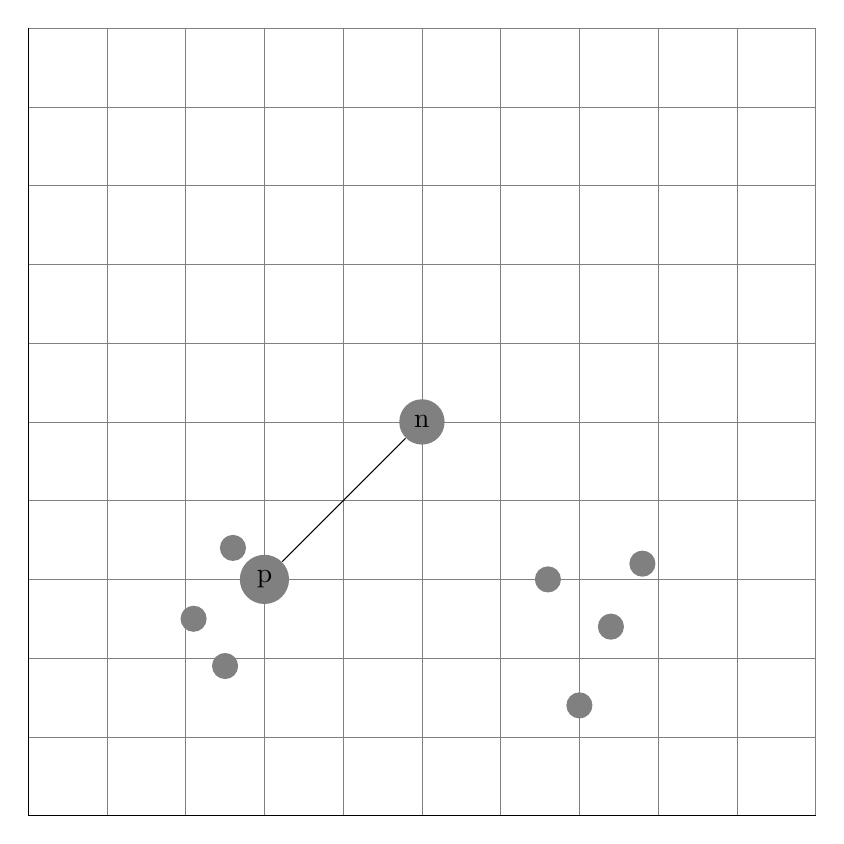
\begin{tikzpicture}
					\draw[help lines] (0,0) grid (10, 10);
					\draw (0,0) -- (0,10);
					\draw (0,0) -- (10,0);

					\node[circle,fill=gray] (p) at (3,3) {p};
					\node[circle,fill=gray] (p2) at (2.1, 2.5) {};
					\node[circle,fill=gray] (p3) at (2.5, 1.9) {};
					\node[circle,fill=gray] (p4) at (2.6, 3.4) {};

					\node[circle,fill=gray] (p5) at (7, 1.4) {};
					\node[circle,fill=gray] (p6) at (7.4, 2.4) {};
					\node[circle,fill=gray] (p7) at (7.8, 3.2) {};
					\node[circle,fill=gray] (p8) at (6.6, 3) {};

					%% outliers
					\node[circle,fill=gray] (n) at (5,5) {n};

					\draw[-] (p) -- (n);
				\end{tikzpicture}
			}
			\end{figure}
		\end{column}

		\begin{column}{0.5\textwidth}
			Overgeneralization, where minority sample $n$ could be an outlier.
		\end{column}
	\end{columns}
\end{frame}


\subsection{LNSMOTE}

%%{{{ LNSMOTE: overview
\begin{frame}{Local-Neighbourhood SMOTE (LNSMOTE)}{Overview}
	LNSMOTE is modification of Safe-Level SMOTE.
	\begin{block}{Safe-level}
		For each minority sample, calculate $k$ number of minority samples in
		their neighbours (k-nearest-neighbourhood -- KNN).

		\begin{itemize}
		\item If number of their neighbors approaching 0, then the sample will
		be considered as noise.
		\item If number of their neighbors approaching $k$ , then the sample is
		in safe region of minority samples.
		\end{itemize}
	\end{block}
\end{frame}
%%}}}

%%{{{ LNSMOTE sl(p) = 0 and sl(n) = 0
\begin{frame}{Local-Neighbourhood SMOTE}{Overview}
	\begin{columns}
		\begin{column}{0.5\textwidth}
			\begin{figure}
			\centering
			\mytikzinput{lnsmote_no_synthetic}
			\resizebox {\columnwidth} {!} {
				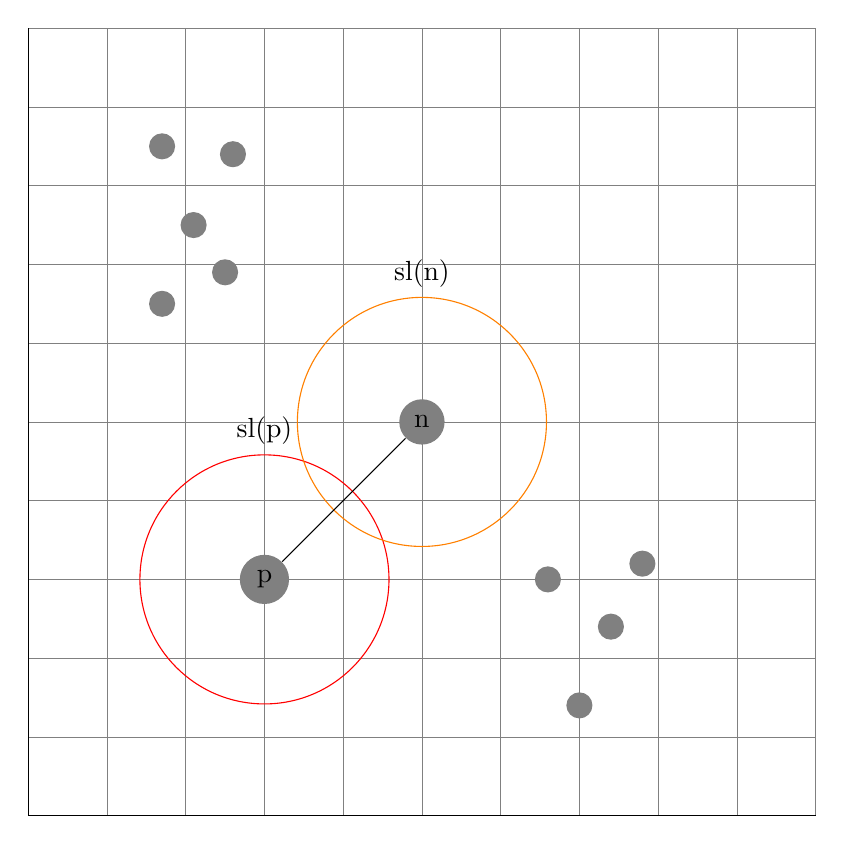
\begin{tikzpicture}
					\draw[help lines] (0,0) grid (10, 10);
					\draw (0,0) -- (0,10);
					\draw (0,0) -- (10,0);

					\node[circle,fill=gray] (p2) at (1.7, 6.5) {};
					\node[circle,fill=gray] (p2) at (1.7, 8.5) {};
					\node[circle,fill=gray] (p2) at (2.1, 7.5) {};
					\node[circle,fill=gray] (p3) at (2.5, 6.9) {};
					\node[circle,fill=gray] (p4) at (2.6, 8.4) {};

					\node[circle,fill=gray] (p5) at (7, 1.4) {};
					\node[circle,fill=gray] (p6) at (7.4, 2.4) {};
					\node[circle,fill=gray] (p7) at (7.8, 3.2) {};
					\node[circle,fill=gray] (p8) at (6.6, 3) {};

					%% outliers
					\node[circle,fill=gray] (p) at (3,3) {p};
					\node[circle,fill=gray] (n) at (5,5) {n};

					\node[circle,
						draw=red,
						minimum width=90pt,
						inner sep=0pt,
						label=sl(p)
					] at (3,3) {};

					\node[circle,
						draw=orange,
						minimum width=90pt,
						inner sep=0pt,
						label=sl(n)
					] at (5,5) {};

					\draw[-] (p) -- (n);
				\end{tikzpicture}
			}
			\end{figure}
		\end{column}

		\begin{column}{0.5\textwidth}
		If safe-level(p) = 0 and safe-level(n) = 0, then both samples is
		considered as noise and no synthetic samples will be created.
		\end{column}
	\end{columns}
\end{frame}
%%}}}

%%{{{ LNSMOTE slp = 1 and sln=0
\begin{frame}{Local-Neighbourhood SMOTE}{Overview}
	\begin{columns}
		\begin{column}{0.5\textwidth}
			\begin{figure}
			\centering
			\mytikzinput{lnsmote_slp1_sln0}
			\resizebox {\columnwidth} {!} {
				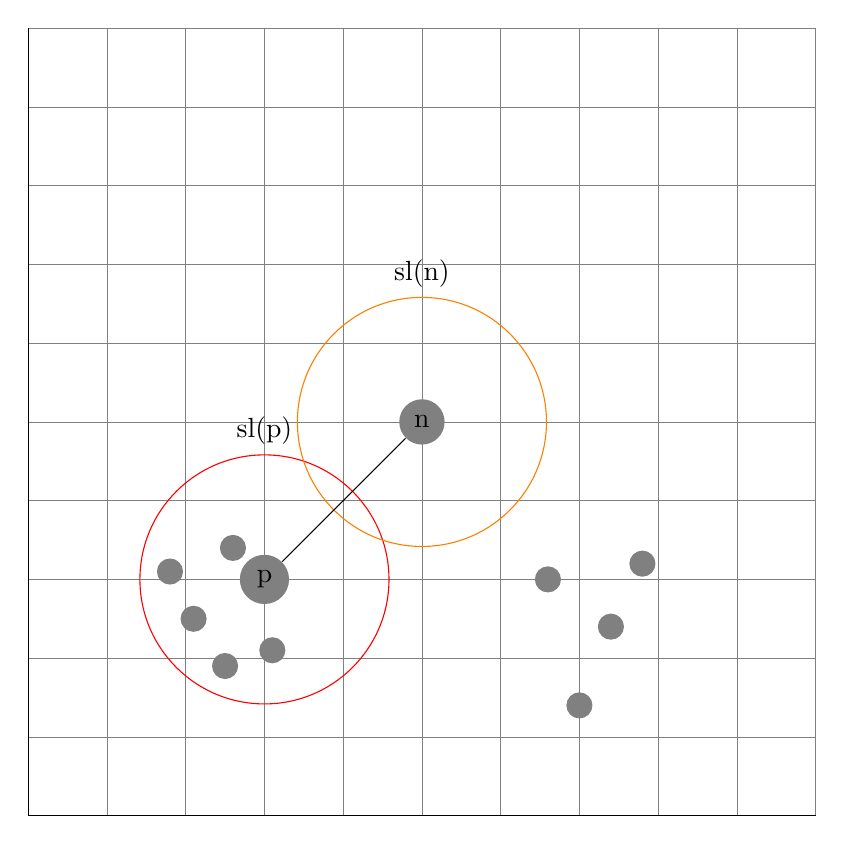
\begin{tikzpicture}
					\draw[help lines] (0,0) grid (10, 10);
					\draw (0,0) -- (0,10);
					\draw (0,0) -- (10,0);

					\node[circle,fill=gray] (p2) at (2.1, 2.5) {};
					\node[circle,fill=gray] (p3) at (2.5, 1.9) {};
					\node[circle,fill=gray] (p4) at (2.6, 3.4) {};
					\node[circle,fill=gray] (p4) at (3.1, 2.1) {};
					\node[circle,fill=gray] (p4) at (1.8, 3.1) {};

					\node[circle,fill=gray] (p5) at (7, 1.4) {};
					\node[circle,fill=gray] (p6) at (7.4, 2.4) {};
					\node[circle,fill=gray] (p7) at (7.8, 3.2) {};
					\node[circle,fill=gray] (p8) at (6.6, 3) {};

					\node[circle,fill=gray] (p) at (3,3) {p};
					\node[circle,fill=gray] (n) at (5,5) {n};

					\node[circle,
						draw=red,
						minimum width=90pt,
						inner sep=0pt,
						label=sl(p)
					] at (3,3) {};

					\node[circle,
						draw=orange,
						minimum width=90pt,
						inner sep=0pt,
						label=sl(n)
					] at (5,5) {};

					\draw[-] (p) -- (n);
				\end{tikzpicture}
			}
			\end{figure}
		\end{column}

		\begin{column}{0.5\textwidth}
		If safe-level(p) = 1 and safe-level(n) = 0, then sample $n$ is a noise
		and synthetic sample will be created by cloning sample $p$.
		\end{column}
	\end{columns}
\end{frame}
%%}}}

%%{{{ LNSMOTE slratio = 1
\begin{frame}{Local-Neighbourhood SMOTE}{Overview}
	\begin{columns}
		\begin{column}{0.5\textwidth}
			\begin{figure}
			\centering
			\mytikzinput{lnsmote_slratio_1}
			\resizebox {\columnwidth} {!} {
				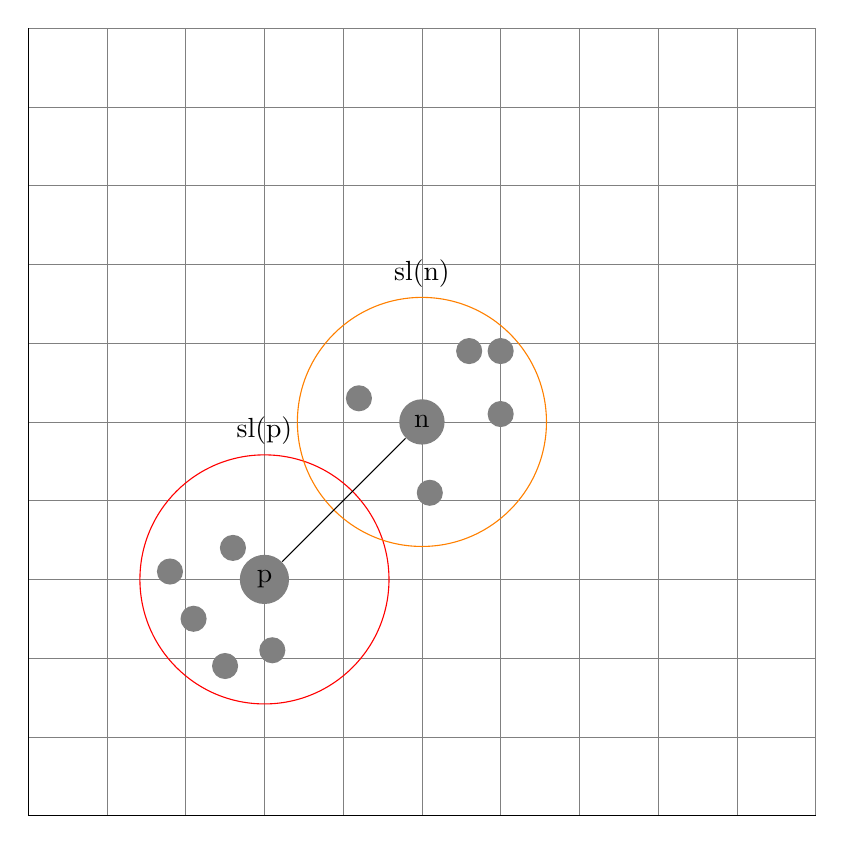
\begin{tikzpicture}
					\draw[help lines] (0,0) grid (10, 10);
					\draw (0,0) -- (0,10);
					\draw (0,0) -- (10,0);

					\node[circle,fill=gray] (p2) at (2.1, 2.5) {};
					\node[circle,fill=gray] (p3) at (2.5, 1.9) {};
					\node[circle,fill=gray] (p4) at (2.6, 3.4) {};
					\node[circle,fill=gray] (p4) at (3.1, 2.1) {};
					\node[circle,fill=gray] (p4) at (1.8, 3.1) {};

					\node[circle,fill=gray] (p5) at (4.2, 5.3) {};
					\node[circle,fill=gray] (p8) at (5.1, 4.1) {};
					\node[circle,fill=gray] (p8) at (5.6, 5.9) {};
					\node[circle,fill=gray] (p8) at (6, 5.9) {};
					\node[circle,fill=gray] (p8) at (6, 5.1) {};

					\node[circle,fill=gray] (p) at (3,3) {p};
					\node[circle,fill=gray] (n) at (5,5) {n};

					\node[circle,
						draw=red,
						minimum width=90pt,
						inner sep=0pt,
						label=sl(p)
					] at (3,3) {};

					\node[circle,
						draw=orange,
						minimum width=90pt,
						inner sep=0pt,
						label=sl(n)
					] at (5,5) {};

					\draw[-] (p) -- (n);
				\end{tikzpicture}
			}
			\end{figure}
		\end{column}

		\begin{column}{0.5\textwidth}
		$ slratio = \frac{safelevel(p)}{safelevel(n)}$ \\
		If $ slratio = 1 $, then synthetic sample will be created like SMOTE.
		\end{column}
	\end{columns}
\end{frame}
%%}}}

%%{{{ LNSMOTE slratio > 1
\begin{frame}{Local-Neighbourhood SMOTE}{Overview}
	\begin{columns}
		\begin{column}{0.5\textwidth}
			\begin{figure}
			\centering
			\mytikzinput{lnsmote_slratio_gt_1}
			\resizebox {\columnwidth} {!} {
				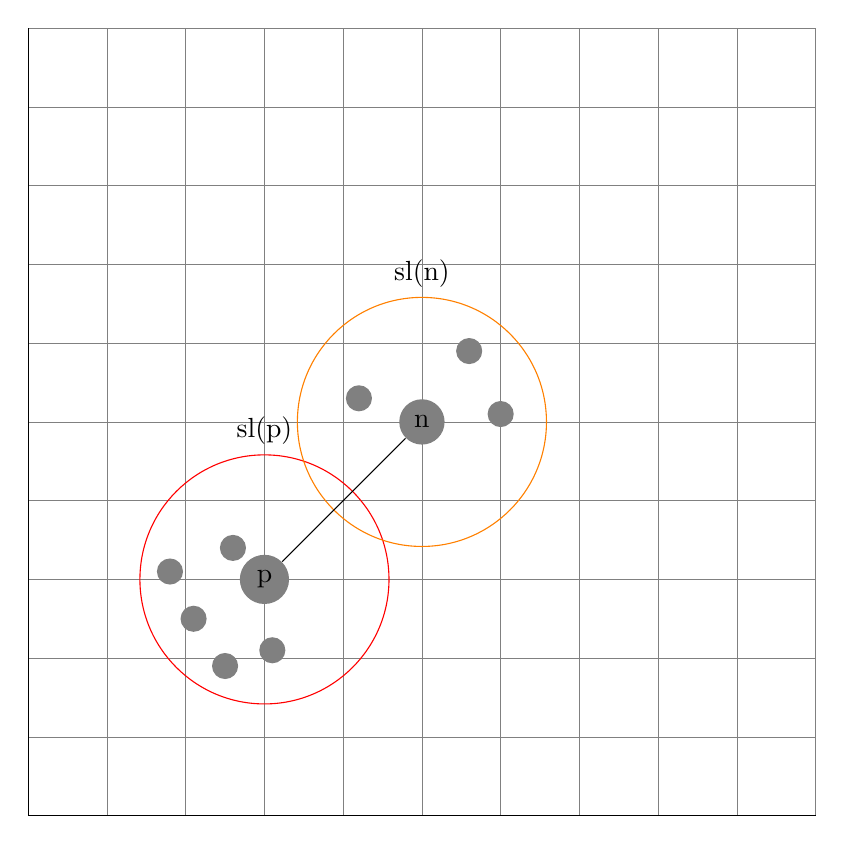
\begin{tikzpicture}
					\draw[help lines] (0,0) grid (10, 10);
					\draw (0,0) -- (0,10);
					\draw (0,0) -- (10,0);

					\node[circle,fill=gray] (p2) at (2.1, 2.5) {};
					\node[circle,fill=gray] (p3) at (2.5, 1.9) {};
					\node[circle,fill=gray] (p4) at (2.6, 3.4) {};
					\node[circle,fill=gray] (p4) at (3.1, 2.1) {};
					\node[circle,fill=gray] (p4) at (1.8, 3.1) {};

					\node[circle,fill=gray] (p5) at (4.2, 5.3) {};
					\node[circle,fill=gray] (p8) at (5.6, 5.9) {};
					\node[circle,fill=gray] (p8) at (6, 5.1) {};

					\node[circle,fill=gray] (p) at (3,3) {p};
					\node[circle,fill=gray] (n) at (5,5) {n};

					\node[circle,
						draw=red,
						minimum width=90pt,
						inner sep=0pt,
						label=sl(p)
					] at (3,3) {};

					\node[circle,
						draw=orange,
						minimum width=90pt,
						inner sep=0pt,
						label=sl(n)
					] at (5,5) {};

					\draw[-] (p) -- (n);
				\end{tikzpicture}
			}
			\end{figure}
		\end{column}

		\begin{column}{0.5\textwidth}
		If $ slratio > 1 $, its mean $p$ is in safe domain within minority
		class, then synthetic sample will be created near $p$ with random gap
		between $[0,1/slratio]$.
		\end{column}
	\end{columns}
\end{frame}
%%}}}

%%{{{ LNSMOTE slratio < 1
\begin{frame}{Local-Neighbourhood SMOTE}{Overview}
	\begin{columns}
		\begin{column}{0.5\textwidth}
			\begin{figure}
			\centering
			\mytikzinput{lnsmote_slratio_lt_1}
			\resizebox {\columnwidth} {!} {
				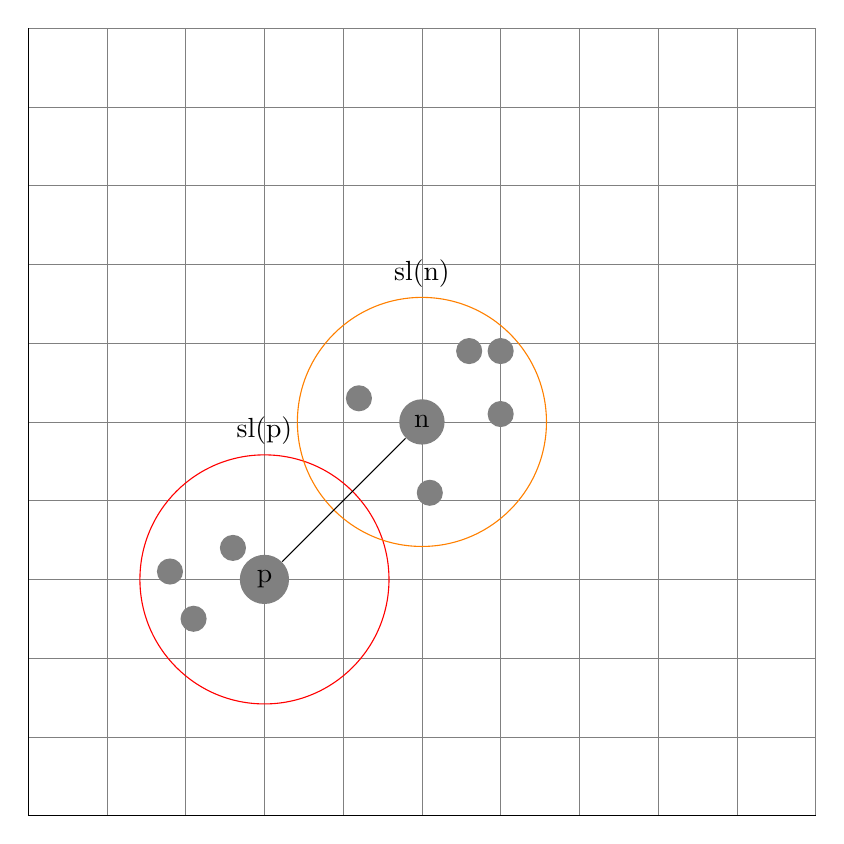
\begin{tikzpicture}
					\draw[help lines] (0,0) grid (10, 10);
					\draw (0,0) -- (0,10);
					\draw (0,0) -- (10,0);

					\node[circle,fill=gray] (p2) at (2.1, 2.5) {};
					\node[circle,fill=gray] (p4) at (2.6, 3.4) {};
					\node[circle,fill=gray] (p4) at (1.8, 3.1) {};

					\node[circle,fill=gray] (p5) at (4.2, 5.3) {};
					\node[circle,fill=gray] (p8) at (5.1, 4.1) {};
					\node[circle,fill=gray] (p8) at (5.6, 5.9) {};
					\node[circle,fill=gray] (p8) at (6, 5.9) {};
					\node[circle,fill=gray] (p8) at (6, 5.1) {};

					\node[circle,fill=gray] (p) at (3,3) {p};
					\node[circle,fill=gray] (n) at (5,5) {n};

					\node[circle,
						draw=red,
						minimum width=90pt,
						inner sep=0pt,
						label=sl(p)
					] at (3,3) {};

					\node[circle,
						draw=orange,
						minimum width=90pt,
						inner sep=0pt,
						label=sl(n)
					] at (5,5) {};

					\draw[-] (p) -- (n);
				\end{tikzpicture}
			}
			\end{figure}
		\end{column}

		\begin{column}{0.5\textwidth}
		If $ slratio < 1 $, its mean sample
		$n$ is in safe domain, then synthetic sample will be created near $n$
		with random gap between $[1-slratio, 1]$.
		\end{column}
	\end{columns}
\end{frame}
%%}}}

\subsection{Random Forest}

\begin{frame}{Random Forest}{Overview}
	\begin{definition}
	Combination of $T$ independent decision tree, such that each tree built
	using $b$ random samples and $m$ random features with the same distribution
	for all trees in the forest.
	\end{definition}
\end{frame}

\begin{frame}
	{Random Forest}
	{Example of Bootstrap Strategy for One Tree}
	\begin{figure}
		\centering
		\mytikzinput{rf_bootstrap_strategy}
		\resizebox {5cm} {!} {
		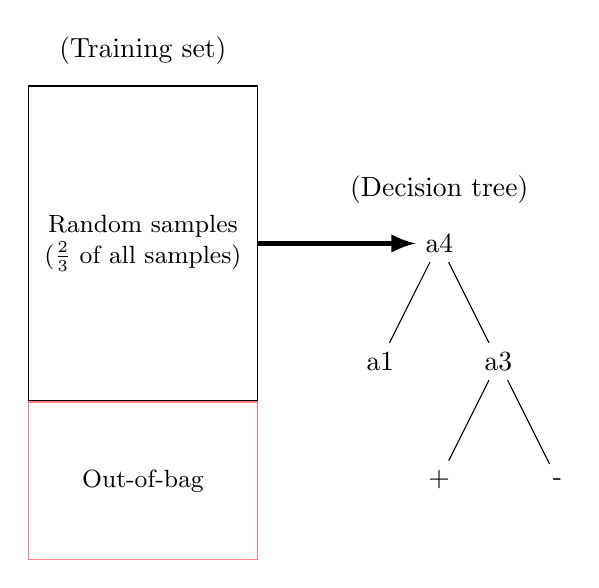
\begin{tikzpicture}[
			nodes = {
				align = center
			},
			block/.style={
				draw,
				fill=white,
				rectangle,
				minimum width={width("Bootstrap samples")+2pt},
				font=\small
			},
			lines/.style={
				line width=2pt,
				>=latex
			}
		]
			\node[block,minimum height=4cm] (bs) {
				Random samples\\
				($\frac{2}{3}$ of all samples)
			};

			\node (l) [above=4pt of bs] {(Training set)};

			\node[block,draw=red!50,minimum height=2cm]
				(oob)
				[below=0cm of bs]
				{Out-of-bag};

			\node (tree) [right=2cm of bs] {a4}
				child {node {a1}}
				child {node {a3}
					child {node {+}}
					child {node {-}}
				};

			\node (ltree) [above=4pt of tree] {(Decision tree)};

			\draw[lines,->] (bs) -- (tree);
		\end{tikzpicture}
		}
	\end{figure}
\end{frame}

\begin{frame}
	{Random Forest}
	{Disadvantages}
	\begin{itemize}
		\item For a large dataset (e.g. greater than 10.000 samples), the time
		required for training the classifier can take several hours.
		\item Random Forest tends to prefer the majority class when used for
		training imbalanced data \cite{strobl2007bias}
		\item After learning several trees Random Forest optimally adapts to
		the training set reaching perfect splits. Hence, the classifier can
		neither improve the detection sensitivity nor reduce the false positive
		rate \cite{baumann2013cascaded}.
	\end{itemize}
\end{frame}

\begin{frame}
	{Random Forest}
	{Disadvantages}
	\begin{columns}
		\begin{column}{0.5\textwidth}
			\begin{figure}
				\centering
				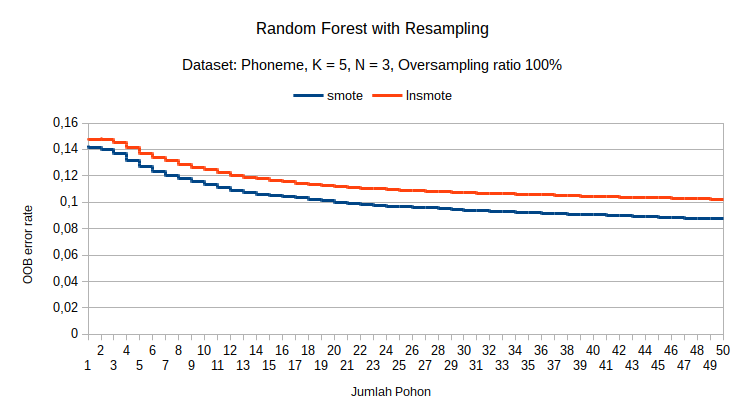
\includegraphics[width=\textwidth]{rf_with_resampling_phoneme}
			\end{figure}
		\end{column}
		\begin{column}{0.5\textwidth}
			After learning several trees, Random Forest optimally adapts to the
			training set reaching perfect splits.
			Hence, the classifier can neither improve the detection sensitivity
			nor reduce the false positive rate \cite{baumann2013cascaded}.
		\end{column}
	\end{columns}
\end{frame}


\subsection{Cascaded Random Forest}

\begin{frame}{Cascaded Random Forest (CRF)}
	{Overview}
	CRF is inspired by cascade structure \cite{viola2004robust}.

	\begin{block}{Cascaded Structure}
		\begin{itemize}
		\item Motivated by assumption that its more easy to reject a negative
		sample than finding a positive one.
		\item Cascaded is combination of classifier in several independent
		stages with the condition that any stage can reject a sample
		\item In order to accept a sample (as positive) all stage must be
		passed.
		\end{itemize}
	\end{block}
\end{frame}

\begin{frame}
	{Cascaded Random Forest (CRF)}
	{Overview}
	\begin{itemize}
		\item A cascade classifier consist of several stages
		\item Each stage contains at least one decision tree
		\item Tree are added until a given true-positive and true-negative rate
		is achieved.
		\item Using aggregated bootstrap strategy.
	\end{itemize}
\end{frame}

\begin{frame}
	{Cascaded Random Forest (CRF)}
	{Bootstrap Strategy}

	\begin{figure}
		\centering
		\mytikzinput{crf_bootstrap_strategy}
		\resizebox {!} {2.5cm} {
		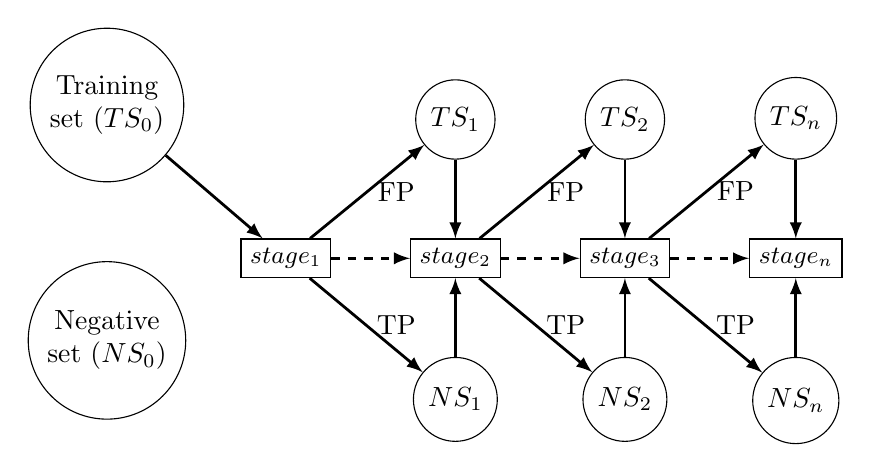
\begin{tikzpicture}[
			nodes = {
				align = center
			},
			data/.style={
				circle,
				draw=black,
				text centered
			},
			block/.style={
				draw,
				fill=white,
				rectangle,
				font=\small
			},
			lines/.style={
				line width=1pt,
				>=latex
			}
		]
			\node[block] (s1) {$stage_1$};
			\node[block] (s2) [right=of s1] {$stage_2$};
			\node[block] (s3) [right=of s2] {$stage_3$};
			\node[block] (sn) [right=of s3] {$stage_n$};

			\node[data] (ts) [above left=of s1] {Training\\set ($TS_0$)};
			\node[data] (ns) [below=of ts] {Negative\\set ($NS_0$)};

			\node[data] (ts1) [above=of s2] {$TS_1$};
			\node[data] (ns1) [below=of s2] {$NS_1$};

			\node[data] (ts2) [above=of s3] {$TS_2$};
			\node[data] (ns2) [below=of s3] {$NS_2$};

			\node[data] (tsn) [above=of sn] {$TS_n$};
			\node[data] (nsn) [below=of sn] {$NS_n$};

			\draw[lines,dashed,->] (s1) -- (s2);
			\draw[lines,dashed,->] (s2) -- (s3);
			\draw[lines,dashed,->] (s3) -- (sn);

			\draw[lines,->] (ts) -- (s1);

			\draw[lines,->] (s1) -- node[right]{TP} ++(ns1);
			\draw[lines,->] (s1) -- node[right]{FP} ++(ts1);

			\draw[lines,->] (ts1) -- (s2);
			\draw[lines,->] (ns1) -- (s2);

			\draw[lines,->] (s2) -- node[right]{TP} ++(ns2);
			\draw[lines,->] (s2) -- node[right]{FP} ++(ts2);

			\draw[lines,->] (ts2) -- (s3);
			\draw[lines,->] (ns2) -- (s3);

			\draw[lines,->] (s3) -- node[right]{TP} ++(nsn);
			\draw[lines,->] (s3) -- node[right]{FP} ++(tsn);

			\draw[lines,->] (tsn) -- (sn);
			\draw[lines,->] (nsn) -- (sn);

		\end{tikzpicture}
		}
	\end{figure}

	\begin{itemize}
		\item After finishing each stage, the classifier then tested using negative
		test set.
		\item Sample that correctly classified as negative will be
		deleted from training set and moved to negative set to be learned by
		the following stage.
		\item Sample that misclassified (false-positive) will be added to
		training set to be learned by the following stage.
	\end{itemize}
\end{frame}

\addtocontents{toc}{\newpage}

\section{Process on Detecting Vandalism}

\begin{frame}
	\begin{multicols}{2}
		\tableofcontents[currentsection]
	\end{multicols}
\end{frame}

\begin{frame}
	{Process on Detecting Vandalism}
	{Overview}
	\begin{figure}[tp!]
\centering
\resizebox{0.3\textwidth}{!} {
\mytikzinput{diagram_process}
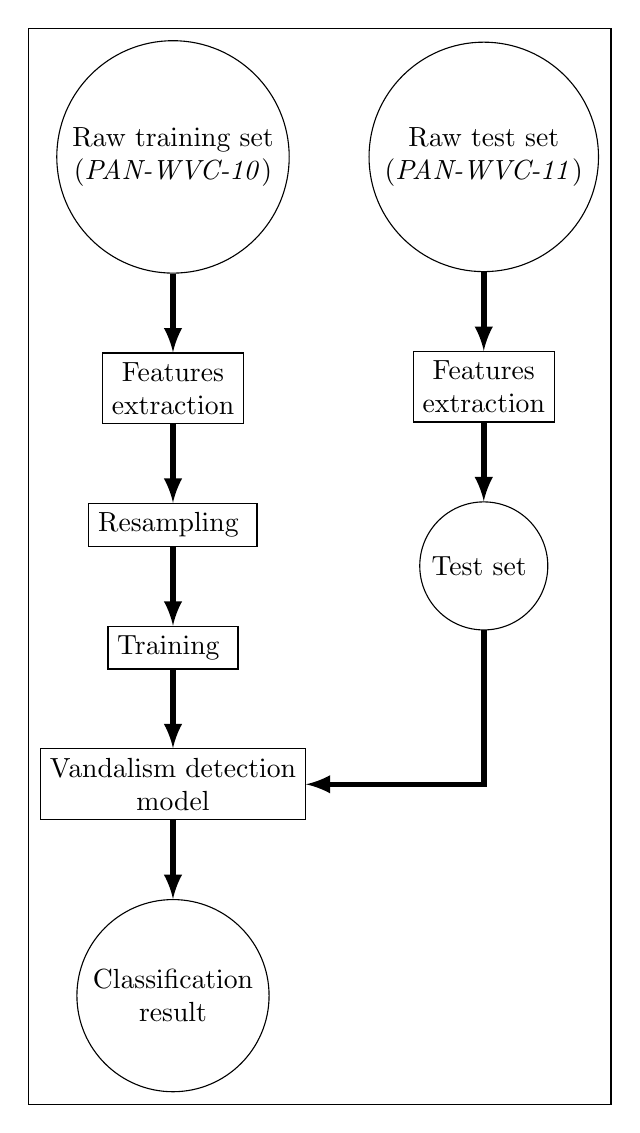
\begin{tikzpicture}[
	framed,
	nodes = {
		align = center
	},
	lines/.style={
		line width=2pt,
		>=latex
	},
	data/.style={
		circle,
		draw=black,
		text centered
	},
	proc/.style={
		rectangle,
		draw=black,
		text centered
	}
]
	\node[data] (training_raw) {
		Raw training set\\
		(\textit{PAN-WVC-10})
	};

	\node[proc] (wvcgen) [below=of training_raw] {
		Features\\
		extraction
	};

	\node[proc] (trainingset) [below=of wvcgen] {
		Resampling
	};

	\node[proc] (c)  [below=of trainingset] {
		Training
	};

	\node[proc] (m)  [below=of c] {
		Vandalism detection\\
		model
	};

	\node[data] (o)  [below=of m] {
		Classification\\
		result
	};
	%%
	\node[data] (testset_raw) [right=of training_raw] {
		Raw test set\\
		(\textit{PAN-WVC-11})
	};

	\node[proc] (testset_wvcgen) [below=of testset_raw] {
		Features\\
		extraction
	};

	\node[data] (testset) [below=of testset_wvcgen] {
		Test set
	};

	\draw[lines,->] (training_raw) -- (wvcgen);
	\draw[lines,->] (wvcgen) -- (trainingset);
	\draw[lines,->] (trainingset) -- (c);
	\draw[lines,->] (c) -- (m);
	\draw[lines,->] (m) -- (o);

	\draw[lines,->] (testset_raw) -- (testset_wvcgen);
	\draw[lines,->] (testset_wvcgen) -- (testset);

	\draw[lines,->] (testset) |- (m);
\end{tikzpicture}
}
\caption{
	Workflow process on detecting vandalism
}
\label{fig:proses}
\end{figure}

\end{frame}

\subsection{Data Preparation}

\begin{frame}{Data Preparation}
	The dataset that we use for training is PAN-WVC-10 and for
	testing is PAN-WVC-11.

	Before we can extract the features, the dataset has to be cleaned and
	modified by
	\begin{itemize}
	\item removing irrelevant attributes, for example \textit{diffurl}
	attribute which contain address in Wikipedia site that referencing current
	sample edit.
	\item Replacing class value with number (i.e. "vandalism" became $1$
	and "regular" became $0$)
	\item Add new attribute "additions" which contains text that was added in
	new revision.
	\item Add new attribute "deletions" which contains text that was deleted in
	old revision.
	\end{itemize}
\end{frame}

\subsection{Features Extraction}

\begin{frame}{Features Extraction}{Overview}
	\begin{itemize}
	\item This paper use 4 metadata features, 11 text features, and 10 language
	features, which based on work of Mola-Velasco.
	\item Features extracted from PAN-WVC-10 and PAN-WVC-11 dataset.
	\end{itemize}
\end{frame}

\begin{frame}{Features Extraction}{Overview}
	\begin{figure}
		\centering
		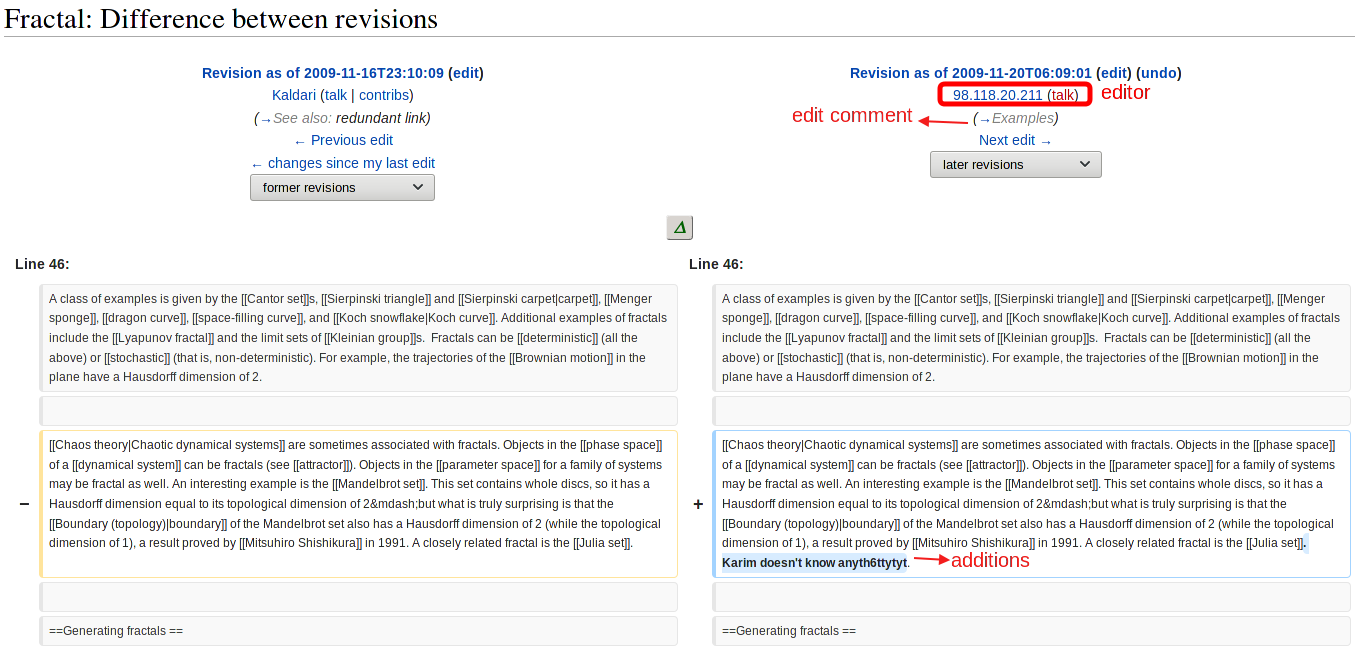
\includegraphics[width=\textwidth]{diff_example}
		\caption{
			Example of edit revision.\\
			(\url{https://en.wikipedia.org/w/index.php?diff=326822930&oldid=326176907})
		}
	\end{figure}
\end{frame}


\begin{frame}
	{Features Extraction}
	{Metadata Features}
	\begin{itemize}
		\item Anonymous. Vandalism usually works of non-registered user.
		\item Comment length. Since this non-registered user does not state why
		or what they changed, they usually leave the comment field empty when
		submitting vandal edit.
		\item Size increment. Absolute decrease in article size can indicated
		deletion, $ newrev - oldrev $
		\item Size ratio.
			$ \frac{1+|newrev|}{1+|oldrev|} $
	\end{itemize}
\end{frame}

\begin{frame}
	{Features Extraction}
	{Text Features}
	\begin{itemize}
		\item Uppercase and lowercase ratio.
			$ \frac{1+|upper|}{1+|lower|} $
		\item Uppercase to all characters ratio.
			$ \frac{1+|upper|}{1+|all|} $
		\item Number ratio.
			$ \frac{1+|number\_chars|}{1+|all|} $
		\item Non-alphanumeric ratio.
			$ \frac{1+|non\-alphanumeric|}{1+|all|} $
		\item Character diversity.
			$ {|all|}^{\frac{1}{1+uniq\-chars}} $
		\item Character distribution. Compute Kullback-Leibler Divergence of
		inserted text to old revision.
	\end{itemize}
\end{frame}

\begin{frame}
	{Features Extraction}
	{Text Features}
	\begin{itemize}
		\item Compression rate. Vandalism usually have low compression rate.
		\item Wiki tokens. Counting the numbers of wiki tokens used in new
		revision, for example \texttt{\_\_TOC\_\_}, \texttt{[Category:]}.
		\item Inserted words frequency.
			$ \sum{\frac{word}{word_{count,newrev}}} $
		\item Longest word length.
		\item Longest character sequence. For example, \textit{aaaarrggg!},
		\textit{soooo huge}.
	\end{itemize}
\end{frame}


\begin{frame}
	{Features Extraction}
	{Language Features}
	\begin{itemize}
		\item Language feature based on number of specific words in certain
		categories.
		\item For each word in categories, two features are calculated for new
		revision:
		frequency and impact.
		\item Frequency is computed by
			$\frac{\textit{word frequency}}
				{\textit{total words}}$
		\item Impact is computed by $\frac{%
				\textit{word frequency in old revision}
			}{
			\textit{word frequency in old revision}
				+ \textit{word frequency in new revision}
			} $
	\end{itemize}
\end{frame}

\begin{frame}
	{Features Extraction}
	{Words Categories}
	\begin{itemize}
		\item Vulgarism contains vulgar and offensive words, for example
		\textit{nigga}, \textit{damn}.
		\item Pronouns contains first and second pronouns words, for example
		\textit{I}, \textit{you}.
		\item Bias contains non-formal words with high bias, for example
		\textit{fabolous}, \textit{lame}.
		\item Pornography contains non-vulgar words that related to
		pornography.
		\item Bad words contains non-vulgar, non-pornography negative words,
		for example \textit{fart}, \textit{smelly}.
		\item All words categories, contains combination of all words.
	\end{itemize}
\end{frame}

\subsection{Resampling}

\begin{frame}
	{Resampling}
	\begin{itemize}
		\item SMOTE resampling parameter: 1,100\% synthetic samples
		\item LNSMOTE resampling parameter: 1,200\% synthetic samples
		\item Both use 5 as KNN value.
	\end{itemize}
	\begin{table}[tp]
\caption{Dataset for training and testing.}
\centering
\begin{tabular}{|| c | l | c | c | c ||}
\hline
\multirow{2}{*}{Type} & \multirow{2}{*}{Resampling mode}
	& \multicolumn{3}{c||}{Number of sample} \\
\cline{3-5}
    & & Vandalism & Regular & Total \\
\hline
\hline
\multirow{3}{*}{Training} & -       &  2.394 & 30.045 & 32.439 \\
                              & SMOTE   & 27.728 & 30.045 & 58.773 \\
                              & LNSMOTE & 28.588 & 30.045 & 58.633 \\
\hline
Testing & - & 1.143 & 8.842 & 9.985 \\
\hline
\end{tabular}
\label{table:dataset}
\end{table}

\end{frame}


\section{Evaluation}

\begin{frame}
	\begin{multicols}{2}
		\tableofcontents[currentsection]
	\end{multicols}
\end{frame}


\subsection{Classifier Parameter}

\begin{frame}
	{Evaluation}
	{Classifier Parameter for Random Forest}
	\begin{block}{Random Forest}
		\begin{itemize}
			\item Number of tree: 200
			\item Percentage of bootstraping: 64\%
			\item Number of random feature: 5
		\end{itemize}
	\end{block}
\end{frame}

\begin{frame}
	{Evaluation}
	{Classifier Parameter for CRF}
	\begin{block}{Common parameters}
		\begin{itemize}
			\item Percentage of bootstraping: 64\%
			\item Number of random feature: 5
			\item True-positive threshold: 0.95
			\item True-negative threshold: 0.95
		\end{itemize}
	\end{block}
	\begin{columns}
		\begin{column}{0.3\textwidth}
			\begin{block}{CRF-200-1}
				\begin{itemize}
					\item Number of stage: 200
					\item Number of tree in each stage: 1
				\end{itemize}
			\end{block}
		\end{column}

		\begin{column}{0.3\textwidth}
			\begin{block}{CRF-100-2}
				\begin{itemize}
					\item Number of stage: 100
					\item Number of tree in each stage: 2
				\end{itemize}
			\end{block}
		\end{column}

		\begin{column}{0.3\textwidth}
			\begin{block}{CRF-50-4}
				\begin{itemize}
					\item Number of stage: 50
					\item Number of tree in each stage: 4
				\end{itemize}
			\end{block}
		\end{column}
	\end{columns}
\end{frame}


\subsection{Classifiers Performance}

\begin{frame}
	{Classifiers Performance}
	{Performance}
	\DTLsetseparator{;}
\DTLloaddb{stats}{./stats.csv}
\DTLmaxforcolumn{stats}{TPR}{\maxtpr}
\DTLminforcolumn{stats}{FPR}{\minfpr}
\DTLmaxforcolumn{stats}{TNR}{\maxtnr}
\DTLmaxforcolumn{stats}{Presisi}{\maxprec}
\DTLmaxforcolumn{stats}{F-Measure}{\maxfm}
\DTLmaxforcolumn{stats}{Akurasi}{\maxacc}
\DTLmaxforcolumn{stats}{AUC}{\maxauc}

\begin{table}[tp]
\caption{Performance of Random Forest and Cascaded Random Forest}
\label{tab:stats}
\centering
\begin{tabular}{llrrrrrrr}
\hline
\textbf{Classifier} &
\textbf{Dataset} &
\textbf{TPR}
\DTLforeach*{stats}{%
	\cl=Klasifikasi,%
	\ds=Dataset,%
	\tpr=TPR%
}{%
	\DTLifnullorempty{\cl}
		{\\ \cline{2-3}}
		{\\ \hline}
	\DTLifnullorempty{\cl}
		{}
		{
			\multirow{3}{2cm}{\cl}
		}
	& \ds
	& \DTLifnumeq{\tpr}{\maxtpr}{\textbf{\tpr}}{\tpr}
}
\\
\hline
\end{tabular}
\end{table}

\end{frame}

\subsection{Computation Time}

\begin{frame}
	{Computation Time}
	{Running Time}
	\DTLloaddb{runtimes}{runtimes.csv}
\begin{table}[bp]
\caption{Training computation time}
\centering
\begin{tabular}{l l r}
\hline
\textbf{Classifier} &
\textbf{Dataset} &
\textbf{Time \newline (minutes)}
\DTLforeach*{runtimes}{%
		\cl=Klasifikasi,
		\ds=Dataset,
		\time=Waktu (menit)%
}{%
	\DTLifnullorempty{\cl}
		{\\ \cline{2-3}}
		{\\ \hline \hline}
	\DTLifnullorempty{\cl}
		{}
		{
			\multirow{3}{2cm}{\cl}
		}
	& \ds
	& \time
}
\\
\hline
\end{tabular}
\label{tab:runtimes}
\end{table}

\end{frame}


\section{Conclusion}

\begin{frame}
	\begin{multicols}{2}
		\tableofcontents[currentsection]
	\end{multicols}
\end{frame}

\begin{frame}
	{Conclusion}
	\begin{itemize}
		\item SMOTE on average increase TPR value by $0.19$ times
		\item LNSMOTE on average increase TPR value $0.33$ times
		\item Overall, the best model for detecting vandalism is CRF with 200
		stages and 1 trees on dataset resampled with LNSMOTE
		\item CRF on average $1.6$ times faster than RF on training resampled
		dataset
	\end{itemize}
\end{frame}

\subsection{Our Contributions}
\begin{frame}
	{Our Contributions}
	\begin{itemize}
		\item A framework to extract vandalism features from Wikipedia dataset
		for speeding up future research or used in real world case.
		(\url{https://github.com/shuLhan/wvcgen})
		\item A framework for LNSMOTE resampling and Cascaded Random Forest
		classifier
		(\url{https://github.com/shuLhan/go-mining})
	\end{itemize}
\end{frame}

\subsection{Future Works}
\begin{frame}
	{Future works}
	\begin{itemize}
		\item Create and collect vandalism annotations for Wikipedia Bahasa
		Indonesia
		\item Parallel algorithm for Random Forest and/or Cascaded Random
		Forest to speeding up process
		\item Experimenting with XGBoost classifier for vandalism detection
	\end{itemize}
\end{frame}

\section*{References}

\begin{frame}{References}
\printbibliography
\end{frame}

\begin{frame}
	{Attribute Partitioning}
	{Gini Index}
	\small
	\begin{algorithmic}[1]
		\Require \\
		$ D $: dataset
		\Function{ComputeGains}{$D$}
			\For{\textbf{each} $A$ \textbf{in} $D$}
				\State $ sortedIdx \gets $ Indirect sort $A$ in asceding
				order
				\State Sort target class $D$ by $ sortedIdx $

				\State $ part \gets [ ] $
				\For{$ i \gets 1,A_{len-1} $}
					\State $ part[i] \gets (A_{i} + A_{i+1}) / 2 $
				\EndFor

				\State $ gini \gets \Call{Gini}{A} $

				\State $ gain \gets [ ] $
				\State $ n \gets A_{len} $
				\For{$ p \gets 1,part_{len} $}
					\State $ gain[p] \gets gini - (
						(\frac{p}{n} \times \Call{Gini}{A_{1,p}})
						+
						(\frac{n - p}{n} \times \Call{Gini}{A_{p,n}})
						)
						$
				\EndFor
			\EndFor
		\EndFunction
	\end{algorithmic}
\end{frame}

\begin{frame}
	{Gini Value}
	\begin{algorithmic}[1]
		\Require \\
		$ T $: subset of dataset \\
		$ m $: classes of dataset
		\Function{Gini}{$T, m$}
			\State \Return{$ 1 - \sum\limits_{x = 1}^{m}
					{(\frac{|C_{x,T}|}{|T|})^2}
					$}
		\EndFunction
	\end{algorithmic}
\end{frame}

\begin{frame}
	{Finding K-nearest-neighbours}
	{Using Euclidian Distance}
	\footnotesize
	\begin{algorithmic}[1]
		\Require \\
		$ S $: samples \\
		$ I $: instance of $S$ to find their neighbors \\
		$ k $: number of neighbors to find
		\Function{FindNeighbors}{$ S, I, k $}
			\State $ nneighbors \gets [] $
			\For{\textbf{each} $s$ \textbf{in} $S$}
				\State $ distance \gets 0 $

				\For{$ x \gets 1,I_{attrs} $}
					\State $ diff \gets I_{x} - s_{x} $
					\State $ distance \gets distance + |diff| $
				\EndFor

				\State Push $s$ and $distance$ to $nneighbors$
			\EndFor

			\State Sort $nneighbors$ in ascending order by their $distance$
			\State $neighbors \gets $ pick top $k$ from $nneighbors$
			\State \Return{$ neighbors $}
		\EndFunction
	\end{algorithmic}
\end{frame}

\end{document}
